\begin{problem}{Golf Time}{standard input}{standard output}{2 seconds}{512 megabytes}

Galina is an aspiring golfer and spends all her free time at a minigolf park. Her favorite golf course in this park is a rectangle, with one of its sides parallel to the north-south direction, and the other one parallel to the east-west direction. The ball is really small and can be considered a point.

Galina wants to practice a specific shot called ``put''. In this shot, a ball is placed somewhere inside the golf course and hit north-east, obtaining the speed of $\sqrt{2}$ inches per second. This means that the ball starts moving by exactly $1$ inch to the north and $1$ inch to the east per second. 

The golf park uses an innovative technology that eliminates all friction, and the ball will continue to move at the initial speed regardless of the traveled distance. Collisions with golf course borders will be perfectly elastic. Fancy!

Inside the course there is a pond that is represented as a simple polygon with edges parallel to the sides of the golf course. If the ball touches the pond, it sinks momentarily.

You are given a list of starting coordinates for Galina's next put training session. For each starting position, assuming a put is shot from this place, calculate how long the ball will travel before falling into the pond and find exactly where it happens, or determine that the ball will move indefinitely.

\InputFile
The first line contains two integers $w$ and $h$, the width and the height of the golf course in inches ($4 \le w, h \le 5 \cdot 10^8$). A coordinate system is introduced in such a way that the corners of the golf course have coordinates $(0, 0)$, $(w, 0)$, $(w, h)$, $(0, h)$, and the point $(1, 1)$ is to the north-east of the point $(0, 0)$.

The second line contains a single integer $n$, denoting the number of vertices in the polygon ($4 \le n \le 1000$).

Each of the following $n$ lines contains two integers $x_i$ and $y_i$, denoting the coordinates of the $i$-th vertex ($1 \le x_i \le w - 1$; $1 \le y_i \le h - 1$). The vertices are listed in traversal order.

All polygon vertices are distinct and none of them lie at the polygon's edge.
All polygon edges are either vertical ($x_i = x_{i+1}$; $x_n=x_1$) or horizontal ($y_i = y_{i+1}$; $y_n=y_1$), and none of them intersects another.

The next line contains a single integer $t$, denoting the number of starting points for a shot ($1 \le t \le 100$).

Each of the following $t$ lines contains two integers $\tilde{x}_i$ and $\tilde{y}_i$, denoting the coordinates of the $i$-th starting point ($1 \le \tilde{x}_i \le w - 1$; $1 \le \tilde{y}_i \le h - 1$). No starting point lies inside or on the border of the pond.

Note that all starting points are independent of each other. In particular, you can assume that there is exactly one ball inside the golf course at any moment.


\OutputFile
For each starting point in order of input, output either a single integer $-1$ if the ball will never sink, or three integers $\tau$ $x_s$ $y_s$, denoting the time before the ball sinks in seconds, and coordinates of the point where it happens ($\tau > 0$; $1 \le x_s \le w - 1$; $1 \le y_s \le h - 1$). Point $(x_s, y_s)$ must belong to the border of the pond.

\Examples

\begin{example}
\exmpfile{example.01}{example.01.a}%
\exmpfile{example.02}{example.02.a}%
\end{example}

\Note
In the first example, the ball trajectories look as shown:

\begin{center}
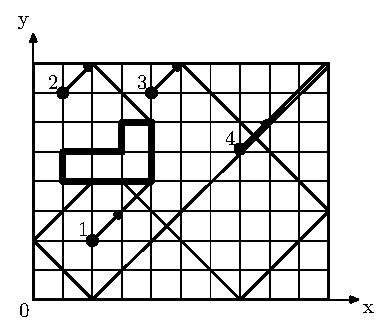
\includegraphics{a-1}
\end{center}

In the second example, starting positions $1$ and $3$ coincide, and for
the position $2$ the ball will never stop:

\begin{center}
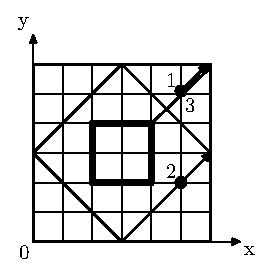
\includegraphics{a-2}
\end{center}

\end{problem}

